\section[参考系]{参~~考~~系}\label{sec:01.04}

牛顿力学所研究的对象是物体的机械运动。从我们日常见到
的车行马跑,及至大到月亮、太阳等星体的运行,小到分子、原子、
粒子的一些飞行,都是属于这一类运动。这类运动的共同特点,
就是物体在空间的位置时刻在变化着。当然,静止的状态、平衡
的状态也是力学的内容之一。

牛顿意义下的运动学,就是研究如何描写物体位置的变化。

\renewcommand{\hsp}{\hspace{0.1em}}
研究问题总是从简单的情况入手。我们首先讨论一种被称为
质点的物体,即大小为零的物体。我们知道,任何具体的物体总
是有一定大小的,没有任何一个物体与质点完全等价。但是,对
于某些特定的运动来说,可以足够准确地把物体看作一个质点。
譬如,在讨论地球绕太阳的公转时,由于地球的半径\hsp(约\hsp 6,400\hsp 公
里)\hsp 比地球与太阳的距离\hsp (约\hsp 149,504,000\hsp 公里)\hsp 小得多,把地球作
为质点是相当好的近似,或者说,在此情况下,将地球作为质点
处理,是一个足够准确的模型。显然,这种模型是有一定适用限
度的。当讨论到地表问题时,再把地球看作质点就大谬不然了。

质点是一个物理对象。对于一个物理对象,用什么数学语言
来描写,这并不是一件很自然的事情,我们知道,任何一种数学
只是一种逻辑体系,一种逻辑体系能不能正确地描写我们的物理
对象,是要认真研究的。物理上,就是要寻找那种能正确地描写
物理对象的数学。在牛顿力学中,质点的空间几何性质,相当于
欧几里德几何上的点。在解析几何中,点的位置是由它的坐标值
来确定的。质点的位置也可以用这种坐标方法来给定。利用坐标
方法,首先要给出坐标系,坐标值总是相对于一定的坐标系而言
的。在数学上,坐标系的选取是完全任意的,但在物理上,我们
要对描写运动的各种物理量进行实际测量,坐标必须固定在一定
\begin{wrapfigure}[11]{l}{48mm}
  %\vspace{-0.5em}
  %\zihao{-5}
  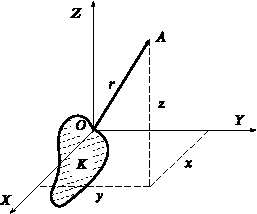
\includegraphics{figure/fig01.04}
  \caption{参考系$K$及参考坐标系$OXYZ$}
  \label{fig:01.04}
  %\vspace{-1.2em}
\end{wrapfigure}
的物体上。例如,如果选取物体$K$上的某点$O$为坐标原点,并选
定$x$,$y$,$z$三个轴,质点$A$的位置即由$x$,$y$,$z$所确定(图\ref{fig:01.04})。
这时,我们称所选取的物体$K$为参考系,而称坐标系$OXYZ$为参
考坐标系。

除了坐标方法外,也可以利用矢量方法来描写质点A的位
置。我们定义质点$A$的位置矢量$\vec{r}$的大小为$OA$的长度,而方向从
$O$指向$A$。用这个矢量就完全确定了质点$A$的位置。在图1.4的坐
标系中,位置矢量$r$的分量就是坐标$x$,$y$,$z$,或写为
\begin{align}\label{eqn:01.04.01}
  \vec{r}=x\vec{i}+y\vec{j}+z\vec{k}
\end{align}
其中$\vec{i}$,$\vec{j}$,$\vec{k}$分别为$X$,$Y$,$Z$轴上的单位矢量,上述两种描述
质点$A$的位置的方法,是完全等价的。

参考系的选择是任意的,可以不用参考系$K$,而用另外一
\begin{wrapfigure}[9]{r}{47mm}
  %\vspace{-0.5em}
  %\zihao{-5}
  
\includegraphics{figure/fig01.05}
  \caption{\ziju{-0.02}从不同参考系观察同一运动}
  \label{fig:01.05}
  %\vspace{-1.2em}
\end{wrapfigure}
个参考系$K'$,譬如,用运动着的车辆来描述质点$A$的位置。由图\ref{fig:01.05}
看到,对干参考系$K$,质点$A$的位置由矢量$\vec{r}$描写,而对于参考
系$K'$,由$\vec{r'}$描写。可见,对于同一个质点的位置,用不同参考系
来描写时,具有不同的位置矢量。就这一点,我们可以说,位
置是具有相对性的物理量。涉及物理量的相对性与绝对性的问题,
以后我们还要专门论述。